\begin{frame}{Facets retrieval}
    \begin{columns}
        \column[T]{0.48\textwidth}
        \begin{figure}
            \centering
            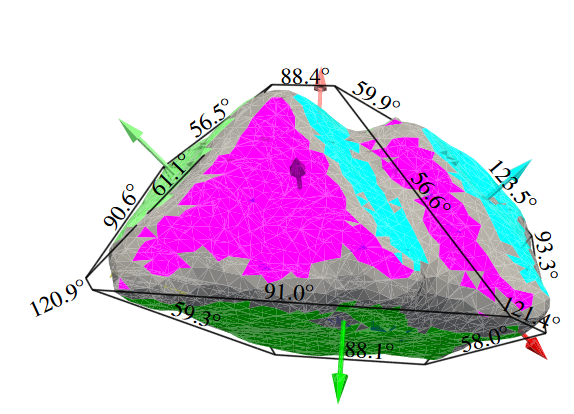
\includegraphics[width=\textwidth]{Figures/bcdi_data/facets_probability.png}
            \caption{A mesh is constructed from the particle voxels }
            \label{fig:particle_mesh}
        \end{figure}

        \column[T]{0.48\textwidth}

        A mesh of the surface is created by the marching-cubes algorithm, resulting in a surface made out of triangles, that in 3D can take up to 26 different orientations. 
        
        The surface is then smoothed to remove the steps created by the voxel size. 

        The main parameters to retrieve the facets are:
        \begin{itemize}
            \item facet normal direction
            \item facet size
            \item roughness tolerance
        \end{itemize}

        The entire procedure has been detailed in literature \footnotemark{}, but could benefit from a Python implementation.

        % Marching square :https://www.sciencedirect.com/topics/computer-science/marching-cube-algorithm
        %These define the tolerance for the roughness of ideally planar facets. 
        %Apart from the determination of the interplanar angles, the relative and absolute facet sizes, the facet normals and centers the main output also labels the faceted regions.
        %The second output of the plugin is an idealized hull of the input, constructed only from the facets found. 
        %The third output consists of the edges of this hull. 
        %Values that belong to two adjacent facets are assigned to these edges, like for example their interplanar angle.
        %The Sample Size, the Angle Uncertainty and the Splat Radius allow to tune the roughness tolerance

        % The Minimum Relative Facet Size allow to reduce the amount of the finally detected facets.

    \end{columns}

    
    \footnotetext{Facet Analyser: ParaView plugin for automated facet detection and measurement of interplanar angles of tomographic objects. Grothausmann, R., Beare, R. (2015) The MIDAS Journal}
\end{frame}